\documentclass{article}[12pt]
\usepackage{fullpage,graphicx, setspace, latexsym, cite,amsmath,amssymb,color,subfigure,mathtools}
%\usepackage{epstopdf}
%\DeclareGraphicsExtensions{.pdf,.eps,.png,.jpg,.mps} 
\usepackage{amssymb} %maths
\usepackage{amsmath} %maths
\usepackage{amsthm}
\usepackage{bbm}
\usepackage{nicefrac}
\usepackage[draft]{commands}

\graphicspath{ {./images/} }

%\newtheorem{theorem}{Theorem}
\newtheorem{prop}{Proposition}
\newtheorem{corollary}{Corollary}
%\newtheorem{lemma}{Lemma}
\newtheorem{defn}{Definition}
\newtheorem{ex}{Example}
\usepackage{float}

\def\R{\mathbf{R}}
\def\Eps{\mathcal{E}}
\def\E{\mathbb{E}}
\def\V{\mathbb{V}}
\def\F{\mathcal{F}}
\def\G{\mathcal{G}}
\def\H{\mathcal{H}}
\def\S{\mathcal{S}}
\def\P{\mathbb{P}}
\def\1{\mathbf{1}}
\def\n{\nappa}
\def\h{\mathbf{w}}
\def\v{\mathbf{v}}
\def\x{\mathbf{x}}
\def\X{\mathcal{X}}
\def\Y{\mathcal{Y}}
\def\eps{\epsilon}
\def\y{\mathbf{y}}
\def\e{\mathbf{e}}



%\def\iid{\sim^{iid}}
%\def\Prob#1{\P[#1]}
%%\def\exp#1{\textup{exp}(#1)}
%\def\mgf{\E\left[e^{\lambda(X-\E X)}\right]}
%\def\Normal{\mathcal{N}}
%\def\Ind#1{\mathbf{1}_{#1}}
%
%\renewcommand{\exp}[1]{\mathrm{exp}\left(#1\right)}
%
%\newcommand{\iid}{\stackrel{\mathclap{\text{\scriptsize{ \tiny i.i.d.}}}}{\sim}}

%\newcommand{\norm}[1]{\left|\left|#1\right|\right|}
%\DeclareMathOperator*{\argmin}{arg\,min}
%\DeclareMathOperator*{\argmax}{arg\,max}

\makeatletter
\newcommand*{\rom}[1]{\expandafter\@slowromancap\romannumeral #1@}
\makeatother



\newcommand{\lecture}[4]{
   \pagestyle{myheadings}
   \thispagestyle{plain}
   \newpage
   % \setcounter{lecnum}{#1}
   \setcounter{page}{1}
   \setlength{\headsep}{10mm}
   \noindent
   \begin{center}
   \framebox{
      \vbox{\vspace{2mm}
    \hbox to 6.28in { {\bf ESE 680-004: Learning and Control
   \hfill Fall 2019} }
       \vspace{4mm}
       \hbox to 6.28in { {\Large \hfill Lecture #1: #2  \hfill} }
       \vspace{2mm}
       \hbox to 6.28in { {\it Lecturer: #3 \hfill Scribes: #4} }
      \vspace{2mm}}
   }
   \end{center}
   \markboth{Lecture #1: #2}{Lecture #1: #2}

   \noindent{\bf Disclaimer}: {\it These notes have not been subjected to the
   usual scrutiny reserved for formal publications. }
   \vspace*{4mm}
}

%notation

\def \E{\mathbb E}
\def \P{\mathbb P}
\def \R{\mathbb R}
\def \A{\cal A}

\begin{document}

\lecture{3}{Concentration Bounds}{Nikolai Matni}{Zongyu Dai}

\vspace{5mm}

The previous lecture focused on identifying the state-space parameters $(A,B,C,D)$ of an unknown linear-time-invariant (LTI) system using \emph{subspace methods}.  Although these methods have been shown to be asymptotically consistent (i.e., up to a similarity transformation, the estimated parameters converge to the true parameters as the number of data points tends to infinity), in this class, we are interested in finite data guarantees.  In particular, we wish to quantify the uncertainty in our estimates as a function of the number of data-points, so that it can then be used as part of a robust control synthesis procedure.  In this lecture, we introduce technical tools known as \emph{concentration bounds}, and show how they can be used to derive exactly these kinds of bounds for a simplified scalar dynamical system.
%This course's pipeline is to combine machine learning algorithms and robust control to provide end-to-end analysis. We need to use some tools to quantify the uncertainty in the output of ML algorithms and we could prove error bounds with high probability. Then we could use those bounds to design control policy. In this lecture, we investigate those technical tools, which are concentration bounds.

\section{Concentration bounds}
\subsection{Bounded Random Variables}
To build some intuition we begin by studying the behavior of almost surely bounded random variables. We assume $\{x_i\}_{i=1}^{N} \iid{} \P^N$, and let $x_i \in [a,b]$ with probability 1.
\newline\\
\begin{theorem}[McDiarmid's Inequality\cite{matni2019tutorial}]
let $x_i \in \X$ for $i=1,2,...,N$ they are independent but not necessarily identical. Then let $F : \X^n \to \R$ satisfies for all $x_1, x_2,...,x_N,x_i^{'} \in \X$
\begin{equation}
\sup_{x_1...x_N,x_i^{'}} {|F(x_1,...,x_N)-F(x_1,...x_{i-1},x_i^{'},x_{i+1},...x_N)|\leq c_i}
\end{equation}
then we have that
\begin{equation}
\Prob{F(x_1,...,x_N)-\E[F(x_1,...,x_N)]\geq t}\leq \exp{-\frac{2t^2}{\sum_{i=1}^n c_i^2}}
\end{equation}
\end{theorem}

\begin{corollary}[Hoeffding's inequality for bounded random variables] Let $\{X_i\}_{i=1}^N \iid p^N$ be such that $X_i \in [a,b]$ a.s..  Then
\begin{equation}
\Prob{\frac{1}{N}\sum_{i=1}^N X_i - \E X_1 \geq t} \leq \exp{\frac{-2Nt^2}{(b-a)^2}}.
\label{eq:hoeff-bound}
\end{equation}
Proof: Set $F(x_1,\dots,x_N) = \frac{1}{N}\sum_{i=1}^N x_i$ and notice that it satisfies the boundedness condition  with $c_i \equiv (b-a)/N$ for all $i$.
\end{corollary}


\begin{ex}
 Let $\{X_i\}_{i=1}^N \iid p^N$ be random vectors in $\mathcal{X}$, and let $\Omega \subseteq \mathcal{X}$ be some set.  Let $\hat{P}_N = \frac{1}{N} \sum_{i=1}^N \Ind{x \in \Omega},$and notice that $\E\hat{P}_N = \Prob{x \in \Omega}$.  As $\Ind{x \in \Omega} \in \{0,1\}$ for all $x$, it follows by equation \eqref{eq:hoeff-bound} that
\begin{equation}
\Prob{\hat{P}_N - \Prob{x \in \Omega} \geq t} \leq \exp{-2Nt^2}.
\end{equation}
We can obtain a similar bound on the probability of the event $\left\{\hat P_N - \Prob{x \in \Omega} \leq -t\right\}$ occurring: it then follows by union bounding over these two events that
\begin{equation}
\Prob{\left|\hat{P}_N - \Prob{x \in \Omega} \right|\geq t} \leq 2\exp{-2Nt^2}.
\end{equation}
\end{ex}
 
 Thus we have seen that in the case of a.s. bounded random variables, concentration of measure does indeed occur.
%  Specifically, we have shown that with high probability,  the empirical mean converges to the true mean at a rate of $O(N^{-1/2})$.  
We will now see that similar concentration occurs for random variables drawn from distributions with sufficiently rapidly decaying tails.  
 
 \subsection{Sub-Gaussian Random Variables}
 We begin by recalling the Chernoff bound, which states that for a random variable $X$ with mean $\E X$, and moment generating function (MGF) $\E\left[e^{\lambda(X-\E X)}\right]$ defined for all $|\lambda|\leq b$, it holds that
 
\begin{equation}
 \log\Prob{X - \E X \geq t} \leq \inf_{\lambda \in [0,b]}\left[\log\E\left[e^{\lambda(X-\E X)}\right] - \lambda t \right].
\label{eq:chernoff}
 \end{equation}
 
 We now turn our attention to Gaussian random variables, and recall that for $X \sim \Normal (\mu,\sigma^2)$, we have that $\E\left[e^{\lambda(X-\mu)}\right]= \exp{\frac{\sigma^2 \lambda^2}{2}}$ for all $\lambda \in \R$.  Substituting this into the Chernoff bound \eqref{eq:chernoff} and solving for $\lambda^\star = t/\sigma^2$, we immediately obtain
\begin{equation}
\Prob{X-\mu \geq t} \leq \exp{\frac{-t^2}{2\sigma^2}}.
\label{eq:gauss-conc}
\end{equation}
 
 
 Recalling that if $X_1 \sim \Normal(\mu_1, \sigma_1^2)$ and $X_2 \sim \Normal(\mu_2,\sigma_2^2)$ then $aX_1+bX_2 \sim \Normal(a\mu_1 + b\mu_2, a^2\sigma_1^2 + b^2 \sigma_2^2)$, it follows immediately that for $X_i \iid \Normal(\mu,\sigma^2)$, it holds that
\begin{equation}
\Prob{\frac{1}{N}\sum_{i=1}^N X_i - \mu \geq t} \leq \exp{\frac{-Nt^2}{2\sigma^2}}.
\label{eq:gauss-mean-prob}
\end{equation}
Once again, a similar bound can be obtained on the probability of event $\left\{\frac{1}{N}\sum_{i=1}^N X_i - \mu \leq -t \right\}$ occurring: it then follows by union bounding over these two events that 
\begin{equation}
\Prob{\left|\frac{1}{N}\sum_{i=1}^N X_i - \mu \right|\geq t} \leq 2\exp{\frac{-Nt^2}{2\sigma^2}}
\label{eq:gauss-mean-deviation}
\end{equation}

We now generalize these results to random variables with MGFs dominated by that of a Gaussian random variable.
 
 \begin{defn}[Sub-Gaussian Random Variable]
A random variable $X$ with mean $\E X$ is sub-Gaussian if there exists a positive number $\sigma^2$ such that
\begin{equation}
\mgf \leq \exp{\frac{\lambda^2\sigma^2}{2}} \ \forall \lambda \in \R.
\label{eq:sub-gauss}
\end{equation}
\label{def:sub-gauss}
\end{defn}
 
 
 An example of random variables that are sub-Gaussian but not Gaussian are bounded random variables -- it can be shown that a random variable $X$ taking values in $[a,b]$ almost surely satisfies equation \eqref{eq:sub-gauss} with parameter $\sigma^2 = (b-a)^2/4$.

Further, from this definition, it follows immediately that from the Chernoff bound that all sub-Gaussian random variables satisfy the concentration bound \eqref{eq:gauss-conc}.  One can also check that if $X_1$ and $X_2$ are sub-Gaussian with parameters $\sigma_1^2$ and $\sigma_2^2$, then $X_1 + X_2$ is sub-Gaussian with parameter $\sigma_1^2 + \sigma_2^2$, from which we immediately obtain Hoeffding's Inequality.
 
 
 \begin{theorem}[Hoeffding's Inequality]
Let $\{X_i\}_{i=1}^N$ be iid sub-Gaussian random variables with parameter $\sigma^2$.  Then
\begin{equation}
\Prob{\frac{1}{N}\sum_{i=1}^N X_i - \E X_1 \geq t} \leq \exp{\frac{-Nt^2}{2\sigma^2}}.
\label{eq:hoeff-subG}
\end{equation}
\label{thm:Hoeffding-subG}
\end{theorem}
 
 
 \paragraph*{An aside on probability inversion and two sided bounds}  Rather than statements about the probability of large deviations, as in bound \eqref{eq:hoeff-subG}, we are often interested in the probability that a random variable concentrates near its mean.  To do so, we employ probability inversion:  if we are willing to tolerate a large deviation occurring with probability at most $\delta$, one may invert bound \eqref{eq:hoeff-subG} by setting $\delta = $ RHS of \eqref{eq:hoeff-subG} and solving for $t$.  This allows us to certify that with probability at least $1-\delta$ that
\begin{equation}
\frac{1}{N}\sum_{i=1}^N X_i \leq  \E X_1 + \sqrt{\frac{2\sigma^2\log(1/\delta)}{N}}.
\end{equation}
Applying the same reasoning to the event $\{X - \E X \leq -t\}$ yields a similar bound, from which it follows, by the union bound, that with probability at least $1-2\delta$ that 
\begin{equation}
\left|\frac{1}{N}\sum_{i=1}^N X_i - \E X_1 \right|\leq \sqrt{\frac{2\sigma^2\log(1/\delta)}{N}}.
\label{eq:two-sided-bound}
\end{equation}
 
 \subsection{Sub-Exponential Random Variables}
 
 Revisiting the error term defined in \eqref{eq:scalar-ols}, we see that we still do not have the requisite tools to perform the desired analysis.

\begin{ex}[Products of Gaussians are not Sub-Gaussian]
Motivated by the error term in \eqref{eq:scalar-ols}, we compute the MGFs for $X^2$ and $XW$, where $X,W\iid \Normal(0,1)$.  Direct computation of the resulting integrals show that
\begin{equation}
\begin{array}{rcl}
\E\left[e^{\lambda(X^2-1)}\right] &=& \frac{e^{-\lambda}}{1-2\lambda}\text{ if $\lambda < 1/2$,} \\
\E\left[e^{\lambda(XW)}\right] &=& \frac{1}{\sqrt{\pi(1-\lambda^2)}}\text{ if $|\lambda|<1$}.
\end{array}
\label{eq:mgfs-for-scalar}
\end{equation}
 These random variables are clearly not sub-Gaussian, as their MGFs do not exist for all $\lambda \in \R$.  However, notice that they can be bounded by the MGF of a Gaussian random variable in a neighborhood of the origin.  In particular we have that
\begin{equation*}
\begin{array}{rcll}
\E\left[e^{\lambda(X^2-1)}\right] &=& \frac{e^{-\lambda}}{1-2\lambda} &\leq \exp{\frac{4\lambda^2}{2}}\text{ $\forall |\lambda| < 1/4$} \\
\E\left[e^{\lambda(XW)}\right] &=& \frac{1}{\sqrt{\pi(1-\lambda^2)}} & \leq \exp{\frac{2\lambda^2}{2}}\text{ $\forall |\lambda|<1/\sqrt{2}$}.
\end{array}
\label{eq:subexp-example}
\end{equation*}
The first inequality follows from some calculus, and the second by leveraging that $-\log(1-x)\leq x(1-x)^{-1}$ for $0 \leq x <1$.
\label{ex:chi-squared}
\end{ex}
 
 
 We now show that MGFs exhibiting behavior as above also concentrate.

\begin{defn}
A random variable $X$ with mean $\E X$ is sub-exponential with parameters $(\nu^2, \alpha)$ if
\begin{equation}
\E\left[e^{\lambda(X-\E X)}\right] \leq \exp{\frac{\nu^2\lambda^2}{2}} \ \forall |\lambda| \leq \frac{1}{\alpha}.
\end{equation}
\label{def:subexp}
\end{defn}

 
 Example \ref{ex:chi-squared} therefore demonstrated that for $X,W \iid \Normal(0,1)$, $X^2$ is sub-exponential with parameters $(4,4)$, and $XW$ is sub-exponential with parameters $(2,\sqrt{2})$. 

\begin{prop}[Sub-exponential tail bound]
if $X$ is sub-exponential with parameters $(\nu^2,\alpha)$, then
\begin{equation}
\Prob{X - \E X \geq t} \leq \begin{cases} \exp{\frac{-t^2}{2\nu^2}}\text{ if $0\leq t \leq \frac{\nu^2}{\alpha}$} \\
\exp{\frac{-t}{2\alpha}}\text{ if $t > \frac{\nu^2}{\alpha}.$}\end{cases}
\label{eq:sub-exp-bound}
\end{equation}

\end{prop}


\textbf{Remark:} Thus we see that for sufficiently small deviations $0\leq t \leq \nu^2/\alpha$, sub-exponential random variables exhibit sub-Gaussian concentration -- indeed, informally, one may view sub-Gaussian random variables as the limit of a sub-exponential random variable with $\alpha \to 0$.  Finally, we note that we can show that for $X_1$ and $X_2$ sub-exponential random variables with parameters $(\nu_i^2,\alpha_i^2)$, we have that $X_1 + X_2$ is a sub-exponential random variable with parameters $(\nu_1^2 + \nu_2^2, \max\{\alpha_1, \alpha_2\})$.  Now we give the proof for this proposition.

\begin{proof} From \cite{wainwright2019high}: by recentering as needed, we may assume without loss of generality that $\mu=0$. We follow the usual Chernoff-type approach: combining it with the definition of a sub-exponential variable yields the upper bound
\[\Prob{X\geq t}\leq e^{-\lambda t}\E[e^{\lambda t}]\leq \exp{-\lambda t+ \frac{\lambda^2\nu^2}{2}} \]
valid for all $\lambda \in [0,\alpha^{-1})$, and we define $g(\lambda, t)=-\lambda t+ \frac{\lambda^2\nu^2}{2}$. In order to complete the proof, it remains to compute, for each fixed $t\geq 0$, the quantity $g^*(t)=\inf_{\lambda \in [0,\alpha^{-1})} g(\lambda, t)$.Note that the unconstrained minimum of the function $g(.,t)$ occurs at $\lambda^* = \frac{t}{\nu^2}$. if $0\leq t\leq \frac{\nu^2}{\alpha}$, then this unconstrained optimum corresponds to the constrained minimum as well, so that $g^*(t)=-\frac{t^2}{2\nu^2}$ over this interval. 

Otherwise, we may assume that $t\geq \frac{\nu^2}{\alpha}$. In this case, since the function $g(.,t)$ is monotonically decreasing in the interval $[0,\lambda^*)$, the constrained minimum is achieved at the boundary point $\lambda'=\alpha^{-1}$, and we have 
\[g^*(t)=g(\lambda',t)=-\frac{t}{\alpha}+ \frac{1}{2\alpha}\frac{\nu^2}{\alpha}\leq -\frac{t}{2\alpha}\]

where the inequality uses the fact that $\frac{\nu^2}{\alpha}\leq t$.
\end{proof}


\vspace{4mm}

As shown in Example 2,the sub-exponential property can be verified by explicitly computing or bounding the moment generating function. This direct calculation may be impracticable in many settings, so it is natural to seek alternative approaches. One such method is based on control of the polynomial moments of variable X. Given a random variable X with mean $\mu = \E [X]$ and variance $\sigma^2 = \E[X^2]-\mu^2$, we say that Bernstein's condition with parameter b holds if 
\begin{equation}
|\E[(X-\mu)^k]| \leq \frac{1}{2}k!\sigma^2 b^{k-2}    \hspace{8mm}     for\hspace{2mm}  k=2,3,4...
\label{eq:Bernstein-condition}
\end{equation}

One sufficient condition for Bernstein's condition to hold is that X be bounded; in particular, if $|X-\mu|\leq b$, then it is straightforward to verify that condition \ref{eq:Bernstein-condition} holds. Even for bounded variables, our next result will show that the Bernstein condition can be used to obtain tail bounds that may be tighter than the Hoeffding bound. Moreover, Bernstein's condition is also satisfied by various unbounded variables, a property which lends it much border applicability.

When X satisfies the Bernstein's condition, then it is sub-exponential with parameters determined by $\sigma^2$ and $b$. Indeed, by  the power-series expansion of the exponential, we have 
\begin{equation}\begin{array}{rcl}
\E[e^{\lambda(X-\mu)}] &=& 1 + \frac{\lambda^2\sigma^2}{2} + \sum_{k=3}^{\infty}\lambda^k\frac{\E[(X-\mu)^k]}{k!}\\ &\leq& 1 + \frac{\lambda^2\sigma^2}{2} +\frac{\lambda^2\sigma^2}{2}\sum_{k=3}^{\infty}(|\lambda|b)^{k-2}

\end{array}
\end{equation}

where the inequality make use of Bernstein's condition. For any $|\lambda|<\frac{1}{b}$, we can sum the geometric series so as to obtain
\begin{equation}
\E[e^{\lambda(X-\mu)}] \leq 1+ \frac{\frac{\lambda^2\sigma^2}{2}}{1-b|\lambda|} \leq e^{\frac{\frac{\lambda^2\sigma^2}{2}}{1-b|\lambda|}}
\label{eq:upper bound}
\end{equation}

where the second inequality follows from the bound $1+t\leq e^t$. Consequently, we conclude that 
\begin{equation}
\E[e^{\lambda(X-\mu)}] \leq e^{\frac{\lambda^2(\sqrt{2}\sigma)^2}{2}}  \hspace{8mm}  for \hspace{2mm}  |\lambda| <\frac{1}{2b}
\end{equation}

As a consequence, an application of sub-exponential tail bound leads directly to tail bounds on a random variables satisfying the Bernstein's condition. However, the resulting tail bound can be sharpened slightly, at least in terms of constant factors, by making direct use of the upper bound \ref{eq:upper bound}. We summarize in the following:
 
 \begin{prop} [Bernstein-type bound] for any random variable satisfying the Bernstein's condition, we have
\[ \mgf \leq e^{\frac{\frac{\lambda^2\sigma^2}{2}}{1-b|\lambda|}}
\hspace{8mm}  for \hspace{2mm}  |\lambda| <\frac{1}{b}\]
and, moreover, the concentration inequality
\[ \Prob{|X-\mu|\geq t}\leq 2e^{-\frac{t^2}{2(\sigma^2+bt)}}
\hspace{8mm}  for \hspace{2mm} t\geq 0\]

\end{prop}
 
 We have proved the first inequality in the discussion preceding this proposition. Using this bound on the moment generating function, the tail bound follows by setting $\lambda = \frac{t}{\sigma^2+bt}\in [0,\frac{1}{b})$ in the Chernoff bound, and then simplifying the resulting expression. 
 
 
 \section{Scalar dynamical system}
 
 Consider the scalar dynamical system
\begin{equation}
x_{t+1} = ax_t + u_t + w_t,
\label{eq:scalar-system}
\end{equation}
for $w_t\iid \Normal(0,\sigma_w^2)$, and $a\in \R$ an unknown parameter.
Our goal is to estimate $a$, and to do so we inject excitatory Gaussian noise via $u_t \iid \Normal (0,\sigma_u^2)$.  We run $N$ experiments over a horizon of $T+1$ time-steps, and then solve for our estimate $\hat{a}$ via the least-squares problem
\begin{equation}\begin{array}{rcl}
\hat{a} &=& \arg\min_a \sum_{i=1}^N (x_{T+1}^{(i)} - ax_{T}^{(i)}- u_T^{(i)})^2\\
&=& a + \frac{\sum_{i=1}^{N}x_T^{(i)} w_T^{(i)}}{\sum_{i=1}^{N} (x^{(i)}_T)^2} =: a + e_N.
\end{array}
\label{eq:scalar-ols}
\end{equation}
Notice that we are using only the last two data-points from each trial -- this simplifies the analysis of the error term $e_N$ greatly as each of the summands in the numerator and denominator are now i.i.d. random variables.  Our goal is to provide high-probability bounds on this error term in this lecture.
 
 
  First, we observe that
\begin{equation} 
 x_T^{(i)} \iid \Normal(0,(\sigma_w^2 + \sigma_u^2) \sum_{t=0}^T a^{2t}).
 \label{eq:scalar-iid-xT}
 \end{equation}
In what follows, we let $\sigma_x^2:= (\sigma_w^2 + \sigma_u^2) \sum_{t=0}^T a^{2t}$, which we recognize as the (variance weighted) finite-time controllability Gramian of the scalar system \eqref{eq:scalar-system}. 

\begin{theorem}
Consider the least squares estimator \eqref{eq:scalar-ols}.  Fix a failure probability $\delta \in (0,1]$, and assume that $N\geq 32 \log(2/\delta)$.  Then with probability at least $1-\delta$, we have that
\begin{equation}
|e_N| \leq 4\frac{\sigma_w}{\sigma_x}\sqrt{\frac{\log(4/\delta)}{N}}.
\end{equation}
\label{thm:iid-scalar-error}
\end{theorem}
 
 
 This theorem follows immediately by invoking the next two propositions with failure probability $\delta/2$ and union bounding.

\begin{proposition}
Fix $\delta \in (0,1]$, and let $N \geq 32 \log(1/\delta)$.  Then with probability at least $1-\delta$
\begin{equation}
\sum_{i=1}^N (x_T^{(i)})^2 \geq \sigma_x^2 \frac{N}{2}.
\label{eq:scalar-iid-lb}
\end{equation}
\label{prop:scalar-iid-lb}
\end{proposition}
\begin{proof}
From \eqref{eq:scalar-iid-xT}, we have that $x_T/\sigma_x \sim \Normal(0,1)$.  Thus from Example \ref{ex:chi-squared}, $x_T^2/\sigma_x^2$ is sub-exponential with parameters $(4,4)$, and 
$\sum_{i=1}^N \left(\nicefrac{x_T^{(i)}}{\sigma_x}\right)^2$
is sub-exponential with parameters $(4N,4)$.  From the tail bound \eqref{eq:sub-exp-bound}, we see that
\begin{align*}
&\Prob{\sigma_x^2\sum_{i=1}^N \left(\frac{x_T^{(i)}}{\sigma_x}\right)^2 - N\sigma_x^2 \leq -t } = \Prob{\sum_{i=1}^N \left(\frac{x_T^{(i)}}{\sigma_x}\right)^2 - N \leq \frac{-t}{\sigma_x^2}} \leq \exp{\frac{-t^2}{8N\sigma_x^4}},
\end{align*}
for all $t \leq N\sigma_x^2$.  Inverting this bound to solve for a failure probability of $\delta$, we see that $t = \sigma_x^2\sqrt{8N\log(1/\delta)} \leq N\sigma_x^2$, where the inequality follows from out assumed lower bound on $N$.  We therefore have, with probability at least $1-\delta$, that
\begin{align*}
\sum_{i=1}^N (x_T^{(i)})^2 \geq \sigma_x^2(N-\sqrt{8N\log(1/\delta)}) \geq \sigma_x^2\frac{N}{2},
\end{align*}
where the final inequality follows from the assumed lower bound on $N$.
\end{proof}

\begin{prop}
Fix $\delta \in (0,1]$, and let $N \geq \tfrac{1}{2} \log(2/\delta)$.  Then with probability at least $1-\delta$
\begin{equation}
\left|\sum_{i=1}^N x_T^{(i)}w_T^{(i)}\right| \leq 2\sigma_x\sigma_w \sqrt{N\log(2/\delta)}.
\label{eq:scalar-iid-ub}
\end{equation}
\label{prop:scalar-iid-ub}
\end{prop}
\begin{proof}
By a similar argument as the previous proof, we have that
$\sum_{i=1}^N \nicefrac{x_T^{(i)}w_T^{(i)}}{\sigma_x\sigma_w}$
is sub-exponential with parameters $(4N,\sqrt{2})$, from which it follows that
\begin{align*}
\Prob{ \left|\sum_{i=1}^N x_T^{(i)}w_T^{(i)}\right| \geq t} &= \Prob{\left|\sum_{i=1}^N \frac{x_T^{(i)}w_T^{(i)}}{\sigma_x\sigma_w}\right| \geq \frac{t}{\sigma_x\sigma_w}} \leq 2\exp{\frac{-t^2}{4N\sigma_x^2\sigma_w^2}},
\end{align*}
if $t\leq 2\sqrt{2}N\sigma_x\sigma_w$.  Inverting with probability failure $\delta$, we obtain $t = 2\sigma_x\sigma_w\sqrt{N\log(2/\delta)} \leq 2\sqrt{2}N\sigma_x\sigma_w$, where the final inequality holds by the assumed lower bound on $N$.  Thus, with probability at least $1-\delta$, \eqref{eq:scalar-iid-ub} holds.
\end{proof}
  
\section{Numerical experiment}

 We use scalar linear system $x_{t+1} = ax_t + u_t + w_t$ to illustrate our bound here. This system has been analyzed in section 2. We set $a=2, T=50,  \delta=0.1, N=100\sim 2100$ and all these experiment numbers  satisfy the inequality $N\geq 32\log(\frac{2}{\delta})$ illustrated in Theorem 3. In both figures, the red line represents true error $e_N$, the blue line represents the error bound we get in Theorem 3. In figure 1, we set $ \sigma_w = \sigma_u = 1  $. In figure 2, we set $ \sigma_w = 1, \sigma_u = 2.  $
  
 \begin{figure}
    \centering
    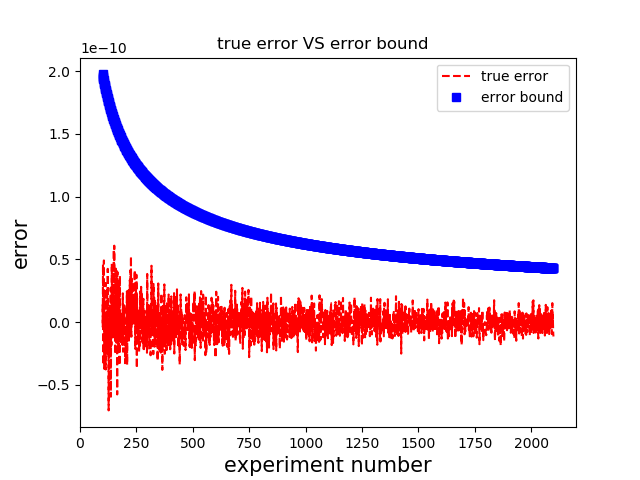
\includegraphics[width = 1.0\textwidth]{1.png}
    \caption{ $\delta_u=1$ $\delta_w=1$ $N=100\sim 2100$, a single experiment has a horizon of 50+1 time-steps, as experiment number increases, we see error bound and true error both converge to 0}
    \label{fig:my_label}
\end{figure}

\begin{figure}
    \centering
    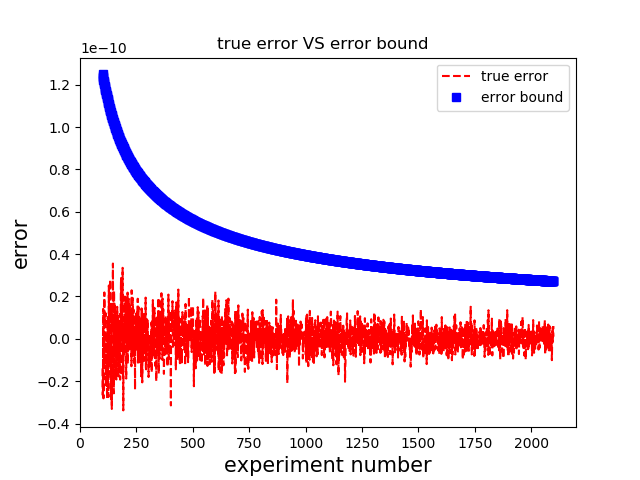
\includegraphics[width = 1.0\textwidth]{2.png}
    \caption{$\delta_u=2$ $\delta_w=1$ $N=100\sim 2100$}
    \label{fig:my_label}
\end{figure}
 
\bibliographystyle{unsrt}
\bibliography{ref}

 
 
 
 
 
 
 
 
 
 
 \end{document}






